\documentclass{article}
\usepackage[utf8]{inputenc}
\usepackage{amsmath}
\usepackage{amssymb}
\usepackage{graphicx}

\newcommand\dm{\mathrm{d}}

\begin{document}
\section*{Periodic Collocation for a Non-Linear Differential Equation}
We are given the following differential equation
\begin{equation*}
    -\frac{\dm^{2}u}{\dm t^{2}}\left(t\right) + u\left(t\right)^{3} = \sin\left(\pi t\right)\,, \quad 0 \leq t < 1
\end{equation*}
We then want to find \textbf{1-periodic} solutions $u : \left[0,1\right] \to \mathbb{C}$ of the above differential equation. We can do this approximately by replacing $u$ with
\begin{equation*}
    u_{N}\left(t\right) := \sum_{j=0}^{N}x_{j}\cos\left(2\pi j t\right) \quad \text{for some } N \in \mathbb{N}
\end{equation*}
and then trying to determine the unknown coefficients $x_{j} \in \mathbb{R}\, \: j = 0, \dots,N$, by solving the \textbf{collocation equations}
\begin{equation*}
    -\frac{\dm^{2}u_{N}}{\dm t^{2}}\left(t_{k}\right) + u_{n}\left(t_{k}\right)^{3} = \sin\left(\pi t_{k}\right) \,,\quad k = 0, \dots, N\,,\quad t_{k} := \frac{k}{N +1}
\end{equation*}
\subsection*{8-16.a}
We are now tasked with writing an efficient \verb|C++| function for given parameters \textit{v} (a vector containing the coefficients $x_{j}$) and an integer $M > N$ which returns the vector 
\begin{equation*}
    \left[u_{N}\left(\frac{k}{m}\right)\right]_{k=0}^{M-1} \in \mathbb{R}^{M}
\end{equation*}
Efficient means that the computational cost must be $\mathcal{O}\left(M\log\left(M\right)\right)$.  We see that the problem for the computational cost is the computation of $u_{N}\left(t\right)$. Looking at the sum
\begin{equation*}
    u_{N}\left(t\right) := \sum_{j=0}^{N}x_{j}\cos\left(2\pi j t\right) \quad \text{for some } N \in \mathbb{N}
\end{equation*}
we can already see some similarity to convolution, furthermore the term $M\log\left(M\right)$ instead of $M^{2}$, which would be the runtime of a naive computation (keeping in mind that $N \cdot M \in \mathcal{O}\left(M^{2}\right)$), also hints at FFT. We are given the hint to use the following equality
\begin{equation*}
    \cos\left(x\right) = \mathsf{Re}\left(e^{-ix}\right)
\end{equation*}

\pagebreak

Remembering the definition of DFT as
\begin{figure}[!hbt]
    \centering
    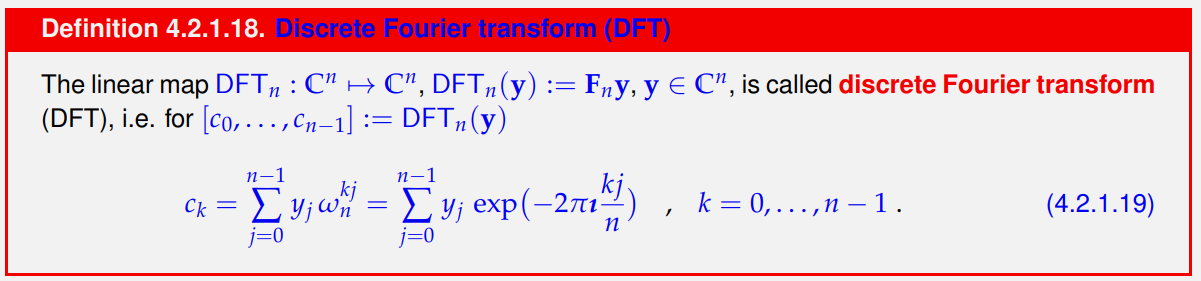
\includegraphics[width=1.0\linewidth]{DFT.png}
\end{figure}
we can see that rewriting the entire equation for $u_N\left(\frac{k}{m}\right)$ gives us
\begin{equation*}
    u_{N}\left(t\right) := \sum_{j=0}^{N}x_{j}\cos\left(2\pi j t\right) = \sum_{j=0}^{N}x_{j}\cdot\mathsf{Re}\left(\text{exp}\left(2\pi i j t\right)\right)
\end{equation*}
Seeing as the input will be of the for $\frac{k}{M}$ be rewrite this to
\begin{equation*}
    u_{N}\left(\frac{k}{M}\right) = \sum_{j=0}^{N}x_{j}\cdot\mathsf{Re}\left(\text{exp}\left(-2\pi i \frac{kj}{M}\right)\right)
\end{equation*}
No we see that this represents a DFT, seeing as our result will be a vector of size $M$, we will apply zero padding to \textit{x}.
\begin{equation*}
    \tilde{\mathbf{x}} = \begin{cases}
        x_{j}\quad &\text{if } j = 1, \dots, N \\
        0 &\text{else}
    \end{cases}
\end{equation*}
We can then use the definition on page $316$ and the code there to implement our function accordingly. It says DFT: \verb|c=fft.fwd(y)|. This gives us the following code.
\begin{figure}[!hbt]
    \centering
    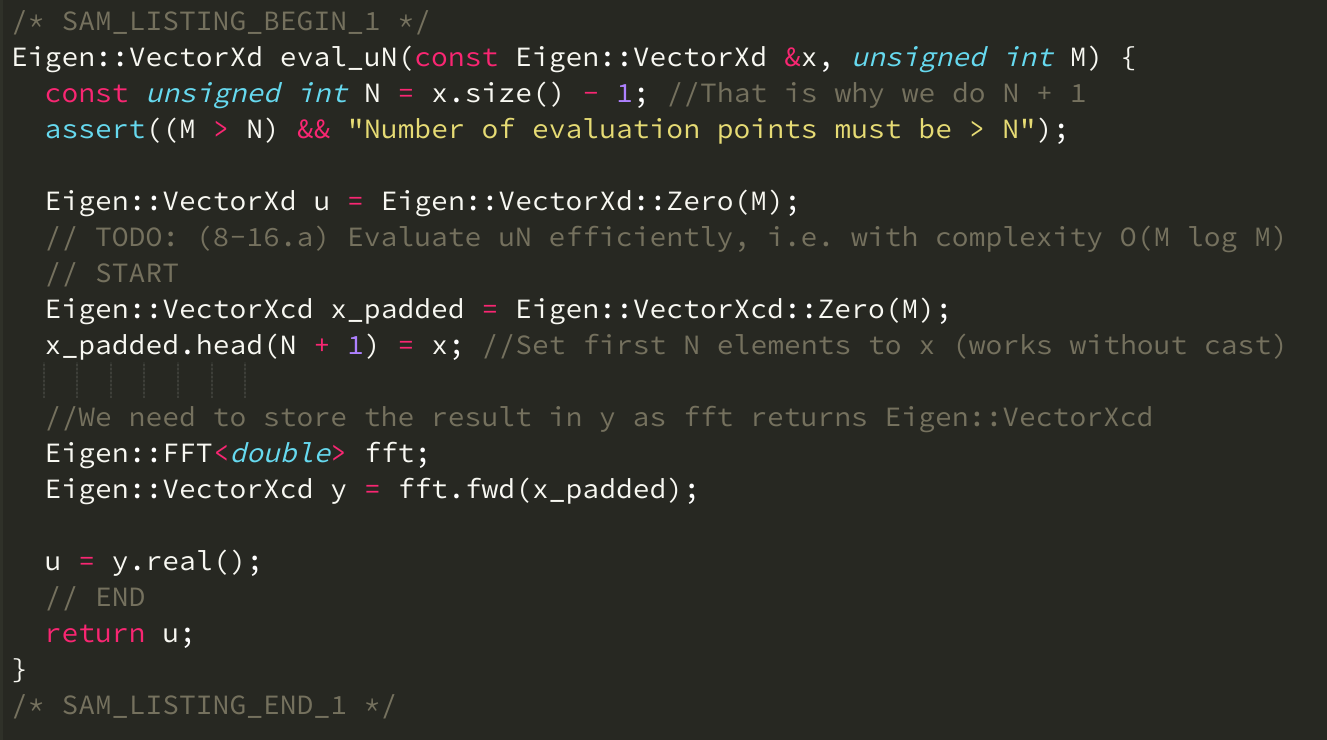
\includegraphics[width=0.9\linewidth]{8-16.a.png}
\end{figure}
\subsection*{8-16.b}
We are now tasked with writing down the collocation equations in the standard form $F\left(\mathbf{x}\right) = \mathbf{0}$. We first rewrite the equations to
\begin{equation*}
   -\frac{\dm^{2}u_{N}}{\dm t^{2}}\left(t_{k}\right) + u_{n}\left(t_{k}\right)^{3} - \sin\left(\pi t_{k}\right) =0 \,,\quad k = 0, \dots, N\,,\quad t_{k} := \frac{k}{N +1} 
\end{equation*}
We can see that we are given exactly $N + 1$ such equations. Hence we set $n = N+1$. The problematic term is the first one given by
\begin{equation*}
     -\frac{\dm^{2}u_{N}}{\dm t^{2}}\left(t_{k}\right) = -\frac{\dm^{2}}{\dm t^{2}}\sum_{j=0}^{N}x_{j}\cos\left(2\pi j t\right)
\end{equation*}
Using the rules of derivation we get
\begin{align*}
    -\frac{\dm^{2}}{\dm t^{2}}\sum_{j=0}^{N}x_{j}\cos\left(2\pi j t\right) &= -\sum_{j=0}^{N}x_{j}\frac{\dm^{2}}{\dm t^{2}}\cos\left(2\pi j t\right) \quad &&\text{(Summation rule)}\\ &= -\sum_{j=0}^{N}x_{j}\frac{\dm}{\dm t}-\sin\left(2\pi j t\right)2\pi j \quad &&\text{(Chain rule)} \\
    &= \sum_{j=0}^{N}x_{j}2\pi j\frac{\dm}{\dm t}\sin\left(2\pi j t\right) \quad \\
    &= \sum_{j=0}^{N}x_{j}2\pi j\cos\left(2\pi j t\right) 2\pi j \quad &&\text{(Chain rule)} \\
    &= \sum_{j=0}^{N}x_{j}4\pi^{2} j^{2}\cos\left(2\pi j t\right)
\end{align*}
So we can write 
\begin{align*}
    F\left(\mathbf{x}\right) &= \left[\sum_{j=0}^{N}x_{j}4\pi^{2} j^{2}\cos\left(2\pi j t_{k}\right) + \left(\sum_{j=0}^{N}x_{j}\cos\left(2\pi j t_{k}\right)\right)^{3} -\sin\left(\pi t_{k}\right)\right]_{k=0}^{N} \\
    &=\left[\sum_{j=0}^{N}x_{j}4\pi^{2} j^{2}\cos\left(2\pi \frac{jk}{N+1}\right) + \left(\sum_{j=0}^{N}x_{j}\cos\left(2\pi \frac{jk}{N+1}\right)\right)^{3} -\sin\left(\pi \frac{k}{N+1}\right)\right]_{k=0}^{N}
\end{align*}
We then have $\mathbf{x} = \left[x_{0}, \dots, x_{N}\right]^{\mathsf{T}}$

\pagebreak

\subsection*{8-16.c}
We are tasked with writing a \verb|C++| function that returns for an input $\mathbf{x}$ the value $\mathbf{F}\left(\mathbf{x}\right)$. We understand how to use $\mathrm{DFT}$ to solve the second term in the equation for $\mathbf{F}\left(\mathbf{x}\right)$, however the first term has a similar structure and we might also be able to use $\mathrm{DFT}$ for it. The term looks like this
\begin{equation*}
    \sum_{j=0}^{N}x_{j}4\pi^{2} j^{2}\cos\left(2\pi \frac{jk}{N+1}\right) = \sum_{j=0}^{N}\left(x_{j}4\pi^{2} j^{2}\right)\cos\left(2\pi \frac{jk}{N+1}\right)
\end{equation*}
We can hence define a vector $\mathbf{y} = \left[4\pi^{2}j^{2}x_{j}\right]_{0}^{N}$ and compute $\mathrm{DFT}_{N}\left(\mathbf{y}\right)$.
This results in the following code.
\begin{figure}[!hbt]
    \centering
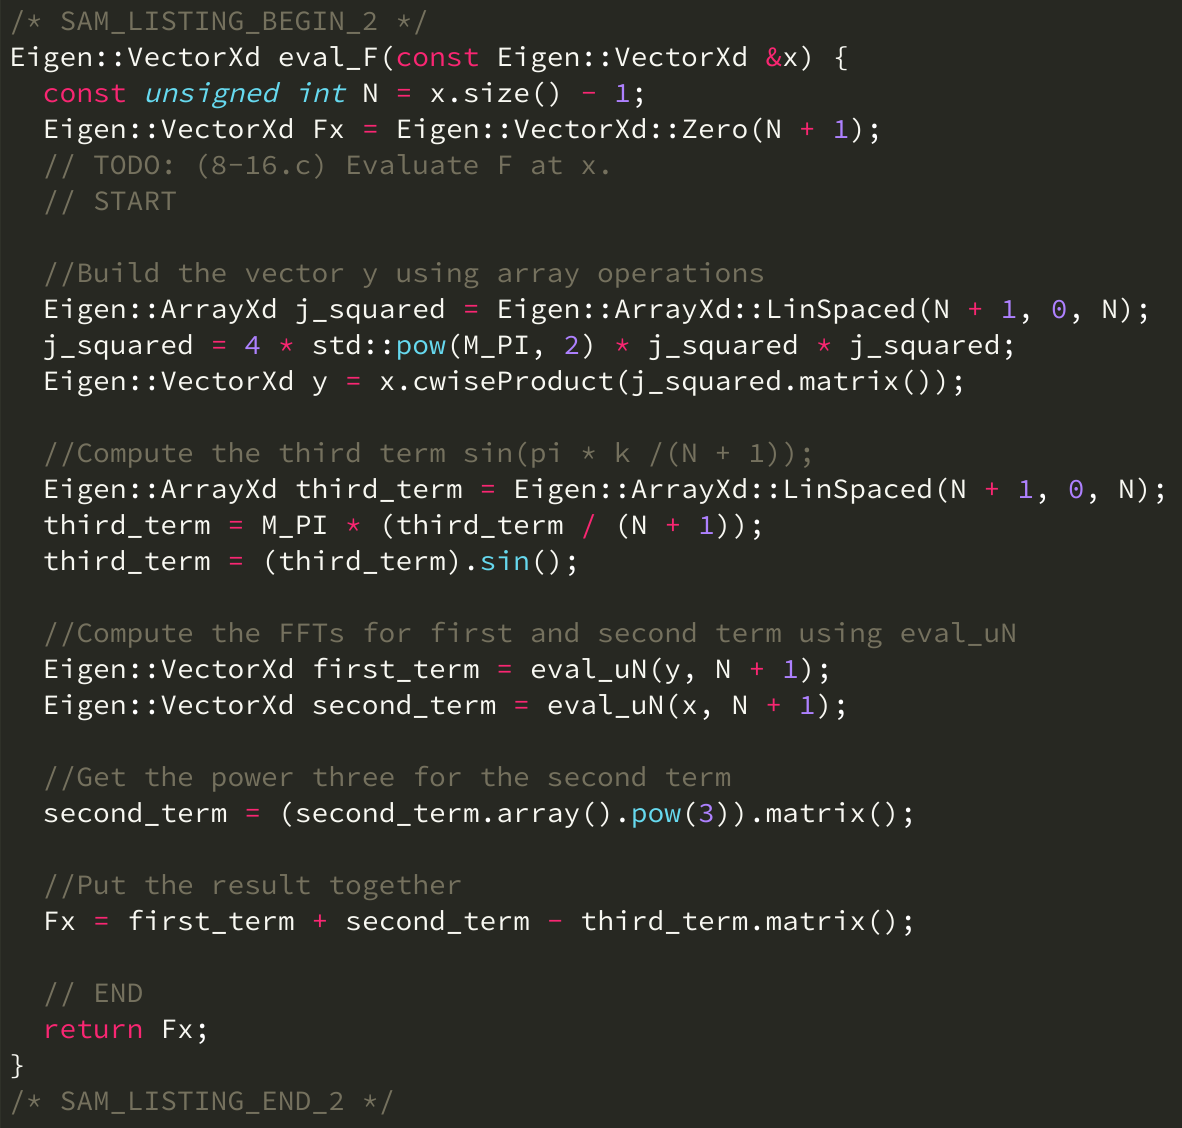
\includegraphics[width=1.0\linewidth]{8-16.c.png}
\end{figure}

\pagebreak

\subsection*{8-16.d} 
We are now tasked to implement a function that evaluates the derivative of $F$. For $F$ we have
\begin{equation*}
F\left(x\right) = \left[\sum_{j=0}^{N}x_{j}4\pi^{2} j^{2}\cos\left(2\pi \frac{jk}{N+1}\right) + \left(\sum_{j=0}^{N}x_{j}\cos\left(2\pi \frac{jk}{N+1}\right)\right)^{3} -\sin\left(\pi \frac{k}{N+1}\right)\right]_{k=0}^{N}
\end{equation*}
We would want to compute the Jacobian of this, i.e.
\begin{equation*}
    \mathrm{D}F\left(x\right) = \left[\frac{\partial F_{k}}{\partial x_{j}}\left(\mathbf{x}\right)\right]_{k,j = 0}^{N}
\end{equation*}
From the notation above we can see that (we need to change $j$ with $l$ as otherwise our summation variable and our derivation variable are the same)
\begin{equation*}
F\left(x\right)_{k} = \sum_{l=0}^{N}x_{l}4\pi^{2} l^{2}\cos\left(2\pi \frac{lk}{N+1}\right) + \left(\sum_{l=0}^{N}x_{l}\cos\left(2\pi \frac{lk}{N+1}\right)\right)^{3} -\sin\left(\pi \frac{k}{N+1}\right)
\end{equation*}
From this we get that
\begin{align*}
    \frac{\partial F_{k}}{\partial x_{j}}\left(\mathbf{x}\right) &= \frac{\partial}{\partial x_{j}}\left(\sum_{l=0}^{N}x_{l}4\pi^{2} l^{2}\cos\left(2\pi \frac{lk}{N+1}\right) + \left(\sum_{l=0}^{N}x_{l}\cos\left(2\pi \frac{lk}{N+1}\right)\right)^{3} -\sin\left(\pi \frac{k}{N+1}\right)\right)  \\
    &= \frac{\partial}{\partial x_{j}}\sum_{l=0}^{N}x_{l}4\pi^{2} l^{2}\cos\left(2\pi \frac{lk}{N+1}\right) + \frac{\partial}{\partial x_{j}}\left(\sum_{l=0}^{N}x_{l}\cos\left(2\pi \frac{lk}{N+1}\right)\right)^{3} -\frac{\partial}{\partial x_{j}}\sin\left(\pi \frac{k}{N+1}\right) \\
    &= 4\pi^{2} j^{2}\cos\left(2\pi \frac{jk}{N+1}\right) + 3\left(\sum_{l=0}^{N}x_{l}\cos\left(2\pi \frac{lk}{N+1}\right)\right)^{2}\left(\cos\left(2\pi \frac{jk}{N+1}\right)\right) \\
    &= \cos\left(2\pi \frac{jk}{N+1}\right)\left(4\pi^{2} j^{2} + 3\left(\sum_{l=0}^{N}x_{l}\cos\left(2\pi \frac{lk}{N+1}\right)\right)^{2}\right)
\end{align*}
Where the third term is a constant in regard to $j$, we used the chain rule for the derivation of the second term and the all terms in the first sum not containing $j$ are treated as constant and thus evaluate to $0$ under derivation. The second term is a candidate for a $\mathrm{DFT}$ (the modified one we implemented in (a)) of the form $\mathrm{DFT}\left(\mathbf{x}\right)$. We hence get the following code. 

\pagebreak

\noindent We will do some optimizations, since we can compute the $\mathrm{DFT}$ beforehand we will do that, we can then compute the power-term once for each $k$ which is the most expensive operation we hence would want to do this only once for each $k$ and thus it makes sense to compute the entries row-wise. This gives us the following code.

\begin{figure}[!hbt]
    \centering
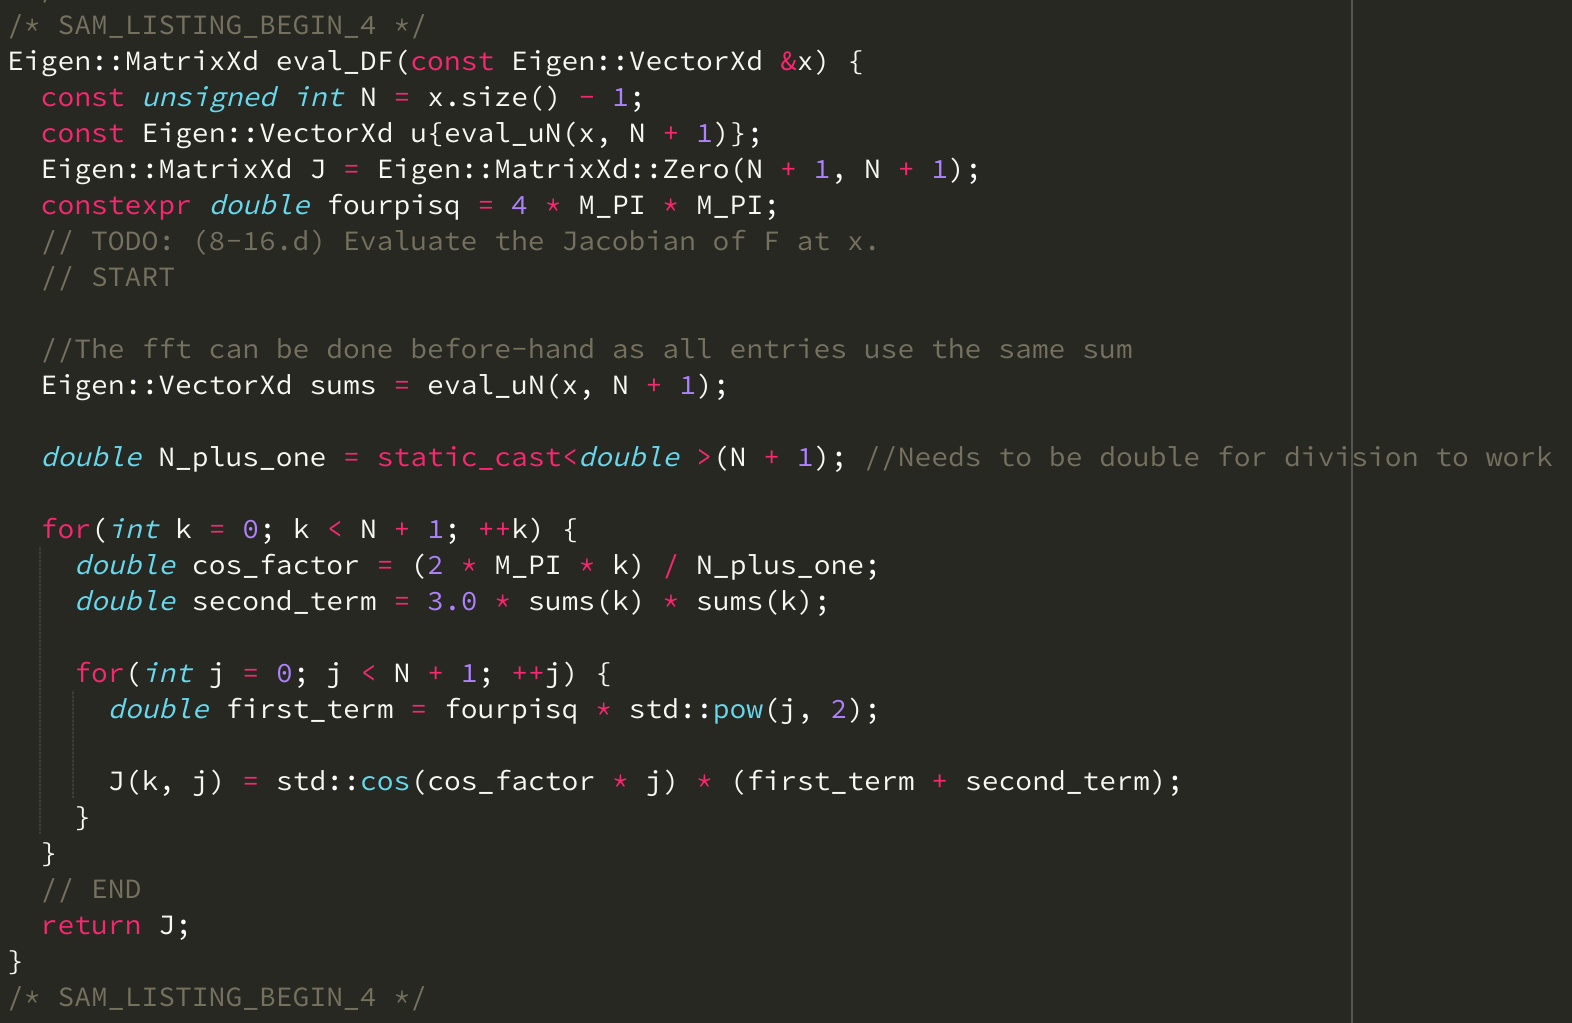
\includegraphics[width=1.0\linewidth]{8-16.d.png}
\end{figure}
\end{document}
